\documentclass[tikz,border=10pt]{standalone}
\usepackage{tikz}
\usetikzlibrary{positioning}

% Global styles for nodes and paths
\tikzset{
  every node/.style={text=black, draw=black, font=\Large, line width=0.5mm},
  every path/.style={draw=black, line width=0.5mm}
}

\begin{document}
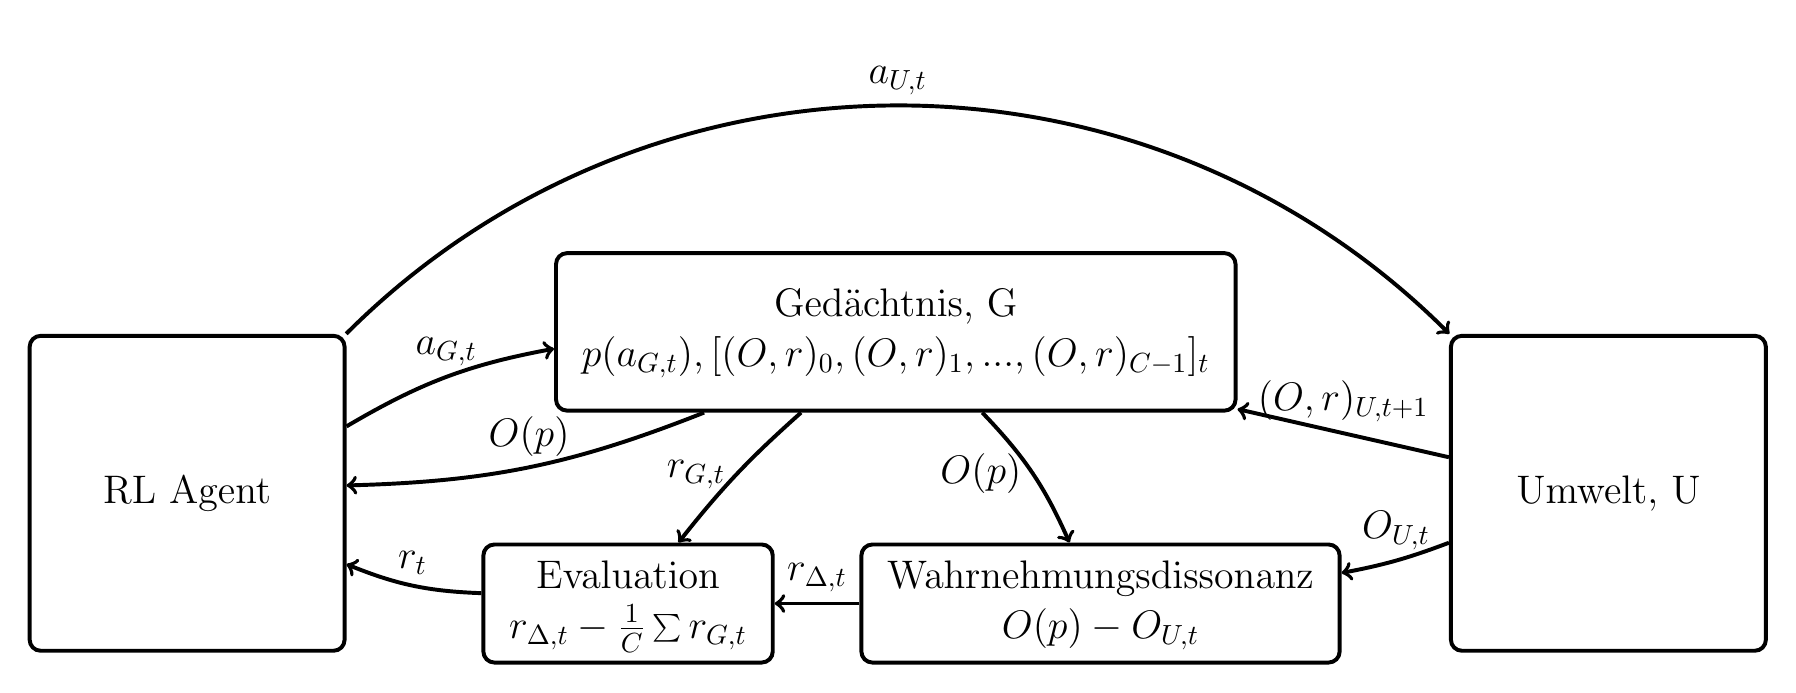
\begin{tikzpicture}[node distance=2cm, auto]
  % Nodes 
  \node (agent) [minimum width=4cm, minimum height=4cm, rounded corners] {RL Agent};
  \node (memory) [above=-1cm of agent, xshift=9cm, minimum width=6cm, minimum height=2cm, rounded corners]  {
    \begin{tabular}{c} Gedächtnis, G \\ $p(a_{G,t}), [(O, r)_0, (O, r)_1, ..., (O, r)_{C-1}]_{t}$ \end{tabular}
  };
  \node (world) [right=14cm of agent, minimum width=4cm, minimum height=4cm, rounded corners] {Umwelt, U};
  \node (evaluator) [rectangle, below=-1.4cm of agent, xshift=5.6cm, rounded corners] {
    \begin{tabular}{c}  Evaluation \\ $r_{\Delta, t} - \frac{1}{C}\sum{r_{G, t}}$ \end{tabular}
  };
  \node (calculator) [rectangle, below=-1.4cm of agent, xshift=11.6cm, rounded corners] {
    \begin{tabular}{c} Wahrnehmungsdissonanz \\ $O(p)-O_{U, t}$ \end{tabular}
  };

  \draw[->] (memory) to[bend left=10] node[midway, above, draw=none, fill=none] {$O(p)$} (agent);
  \draw[->] (memory) to[bend right=5] node[midway, left, draw=none, fill=none] {$r_{G, t}$} (evaluator);
  \draw[->] (world) to[bend left=5] node[midway, above, draw=none, fill=none] {$O_{U, t}$} (calculator);
  \draw[->] (memory) to[bend left=10] node[midway, left, draw=none, fill=none] {$O(p)$} (calculator);
  \draw[->] (calculator) to[bend left=0] node[midway, above, draw=none, fill=none] {$r_{\Delta, t}$} (evaluator);
  \draw[->] (agent) to[bend left=10] node[midway, above, draw=none, fill=none] {$a_{G, t}$} (memory);
  \draw[->] (agent) to[bend left=45] node[midway, above, draw=none, fill=none] {$a_{U, t}$} (world);
  \draw[->] (world) to[bend left=0] node[midway, above, draw=none, fill=none] {$(O, r)_{U, t+1}$} (memory);
  \draw[->] (evaluator) to[bend left=10] node[midway, above, draw=none, fill=none] {$r_t$} (agent);
\end{tikzpicture}
\end{document}